\documentclass{article}
\title{Alternate Pace v2.1}
\author{Peter Todd}
\date{}
\usepackage{graphicx}
\usepackage{url}
\begin{document}
   \maketitle

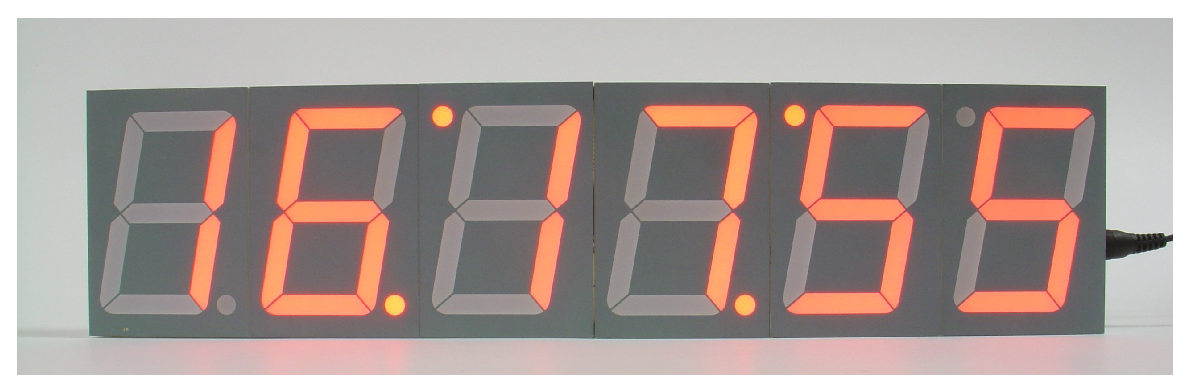
\includegraphics[width=4.25in]{figures/front-running-24hr.eps}

\section{Overview}

The Alternate Pace clock uses the standard definition for the hours and
minutes, however for the seconds the user is given the option of having 120
seconds in a minute, or 30 seconds in a minute, thereby subtly altering the
perception of the passage of time.

\subsection{Specifications}

\begin{itemize}
	\item Dimensions: 11.250" x 2.725" x 0.75"
	\item Accuracy: ${\pm}$2 minutes/year
	\item User interface: Seven segment LED display and push-buttons
	\item Power source: 12VDC 1A wall adapter
	\item Blackout endurance: minimum 24 hours
	\item Internally tracked metrics: Hours meter and user interactions
\end{itemize}

\section{Mounting}

Two slots on the back are provided for hanging. They accept any screw or nail
that fits securely. The distance between the two slots is 9.450" Two power
jacks are also provided; use which ever one best fits the installation.

\section{Setting the time}

As shown in Figure \ref{fig:top-buttons} there are three buttons used for
setting the time, each positioned above the digits that it changes, hours,
minute or seconds. The hours and minutes buttons both increment the associated
digits. Seconds however resets the the seconds to zero. This is provided to
allow you to accurately synchronize the seconds with a master clock by setting
the minutes to be a minute ahead, and then resetting the seconds at the turn of
the minute.

\begin{figure}
\centering
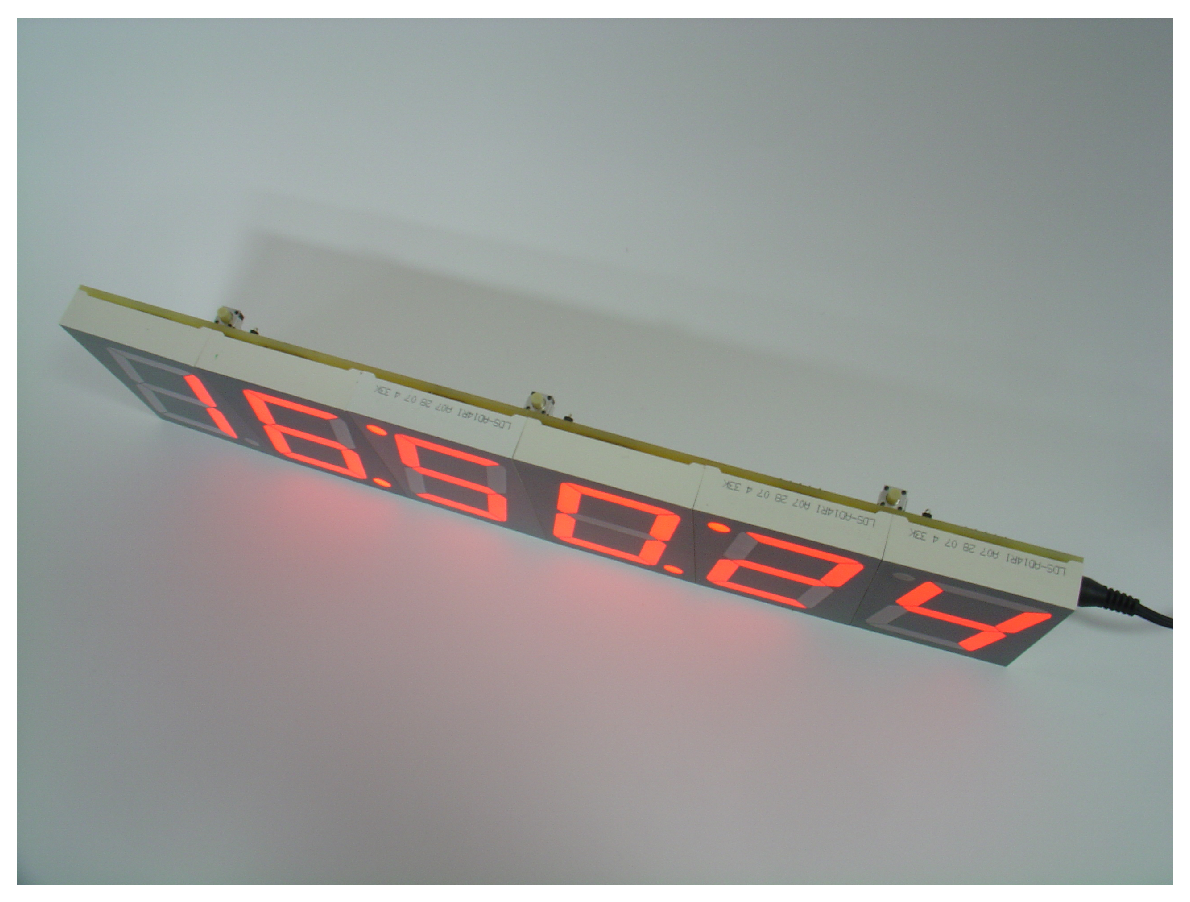
\includegraphics[width=4.75in]{figures/top-buttons.eps}
\caption{Top buttons, hour, minute and second}
\label{fig:top-buttons}
\end{figure}

\pagebreak

\section{12 and 24 hour modes}

To switch between the 12 and 24 hour modes press and hold the hours button.
Note that hours will increment at first, but upon switching modes this
increment will be undone leaving the correct time. In 12 hours mode the bottom
left dot will turn off in the first half of the day to distinguish AM and PM,
as shown in Figure \ref{fig:front-running-12hr-am} The current mode is saved in
non-volatile memory and will be remembered if the power is disconnected.

\begin{figure}
\centering
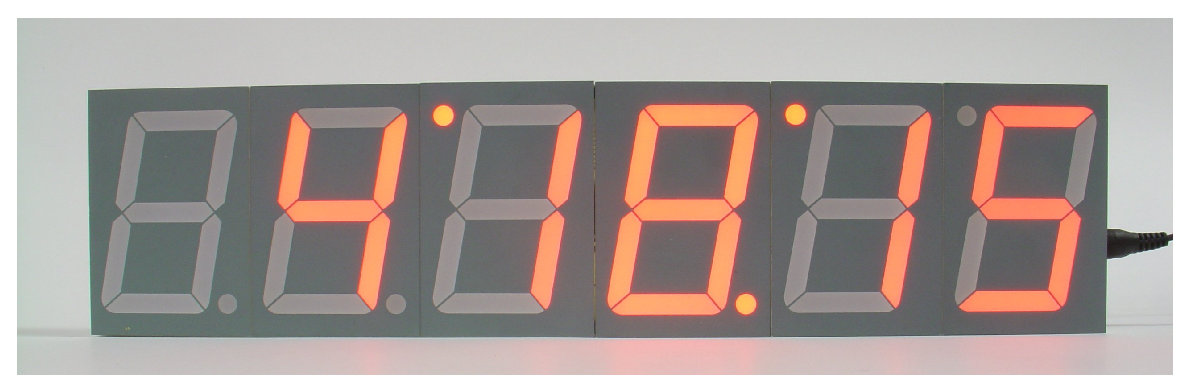
\includegraphics[width=4.75in]{figures/front-running-12hr-am.eps}
\caption{12 hours mode, showing 4am}
\label{fig:front-running-12hr-am}
\end{figure}

\section{Fast and slow modes}

To switch between the fast, 120 seconds in a minute, and slow, 30 seconds in a
minute, modes first disconnect power from the Alternate Pace. Then hold either
the hours, or seconds button down, for slow and fast modes respectively. Now
while holding the buttons down reconnect the power and release the button. You
will see the new mode now. Like the 12/24hour setting, the fast/slow mode is
stored in non-volatile memory and will persist even if power is removed.

\section{Brightness Control}

The brightness of the display can be adjusted via the rotary control labeled
``Bright'' located on the back of the Alternate Pace on the right-hand side.

\section{Maintenance}

The Alternate Pace requires no maintenance. If cleaning is required water
will not harm the electronics so long as the device is off and allowed to dry
throughly before applying power again. It's best to simply use a damp cloth;
free water may become trapped between the led digits and the circuit board and
may take a long time to dry.

\pagebreak

\section{Internal metrics}


The internal metrics permanently record a number of measurements such as the
total time the Alternate Pace has been powered on and how often the buttons
have been pressed. Think of it like the odometer in your car, except, the
Alternate Pace has no need for oil changes.

To access the internal metrics follow the same procedure to switch between fast
and slow modes, except hold down the minutes button on power up. Upon power up
the clock face will display a special mode, shown in Figure \ref{fig:metrics}
In this mode the left most digits, what would normally be hours, display the
address while the right-most digits, normally seconds, display the data at that
address. You can scroll through the addresses with the hours and seconds
buttons. Both address and data digits are in hexadecimal. The table of
addresses and their meanings is as follows:

\medskip

\begin{tabular}{|c|l|r|}
\hline
0x00 - 0x03 & Total running time & In seconds \\ \hline
0x04 - 0x07 & Hours switch & \# of button presses \\ \hline
0x08 - 0x0B & Minutes switch & \# of button presses \\ \hline
0x0C - 0x0F & Seconds switch & \# of button presses \\ \hline
0x10 - 0x13 & Max temperature & \# Raw value from DS3231 \\ \hline
0x14 - 0x17 & Min temperature & \# Raw value from DS3231 \\ \hline
0x18 - 0x1B & Metrics mode usage& \# of times activated\\ \hline
0x1C - 0x1F & Fast/Slow & Fast or slow mode \\ \hline
0x20 - 0x23 & 12/24hr & 12 or 24 hour mode \\ \hline
\end{tabular}

\medskip

Each data value is a 4-byte unsigned integer stored in little-endian format. To
convert this into a human readable decimal integer you'll need a calculator
capable of converting from hexadecimal, or base-16, to base-10. Little-endian
means that the least significant digit is stored in memory first. For instance
the number, 1234 is stored in little endian format as 4321. As an example if
the value in the total running time metric, starting from address zero, was 7b,
c2, 08, 00 you would enter that into your calculator as hexadecimal 0008c27b,
which converted to base-10 is 574075 seconds. Dividing that number by 86400
seconds/day gives you 6.64 days of total running time.

\begin{figure}
\centering
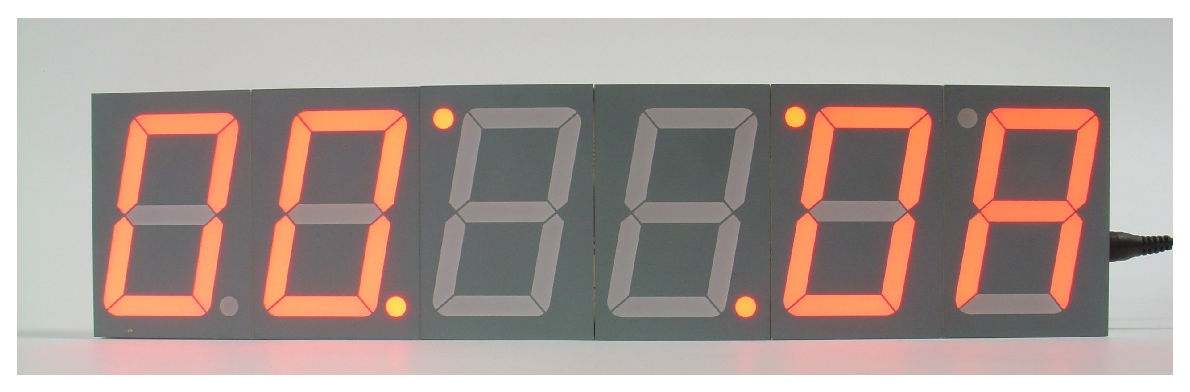
\includegraphics[width=4.75in]{figures/metrics.eps}
\caption{Metrics display}
\label{fig:metrics}
\end{figure}

\end{document}

